\documentclass[11pt,compress,t,notes=noshow, xcolor=table, aspectratio=169]{beamer}
\usepackage[]{graphicx}

\usepackage[]{color}
% maxwidth is the original width if it is less than linewidth
% otherwise use linewidth (to make sure the graphics do not exceed the margin)
\makeatletter
\def\maxwidth{ %
  \ifdim\Gin@nat@width>\linewidth
    \linewidth
  \else
    \Gin@nat@width
  \fi
}
\makeatother

\definecolor{fgcolor}{rgb}{0.345, 0.345, 0.345}
\newcommand{\hlnum}[1]{\textcolor[rgb]{0.686,0.059,0.569}{#1}}%
\newcommand{\hlstr}[1]{\textcolor[rgb]{0.192,0.494,0.8}{#1}}%
\newcommand{\hlcom}[1]{\textcolor[rgb]{0.678,0.584,0.686}{\textit{#1}}}%
\newcommand{\hlopt}[1]{\textcolor[rgb]{0,0,0}{#1}}%
\newcommand{\hlstd}[1]{\textcolor[rgb]{0.345,0.345,0.345}{#1}}%
\newcommand{\hlkwa}[1]{\textcolor[rgb]{0.161,0.373,0.58}{\textbf{#1}}}%
\newcommand{\hlkwb}[1]{\textcolor[rgb]{0.69,0.353,0.396}{#1}}%
\newcommand{\hlkwc}[1]{\textcolor[rgb]{0.333,0.667,0.333}{#1}}%
\newcommand{\hlkwd}[1]{\textcolor[rgb]{0.737,0.353,0.396}{\textbf{#1}}}%
\let\hlipl\hlkwb

\usepackage{framed}
\makeatletter
\newenvironment{kframe}{%
 \def\at@end@of@kframe{}%
 \ifinner\ifhmode%
  \def\at@end@of@kframe{\end{minipage}}%
  \begin{minipage}{\columnwidth}%
 \fi\fi%
 \def\FrameCommand##1{\hskip\@totalleftmargin \hskip-\fboxsep
 \colorbox{shadecolor}{##1}\hskip-\fboxsep
     % There is no \\@totalrightmargin, so:
     \hskip-\linewidth \hskip-\@totalleftmargin \hskip\columnwidth}%
 \MakeFramed {\advance\hsize-\width
   \@totalleftmargin\z@ \linewidth\hsize
   \@setminipage}}%
 {\par\unskip\endMakeFramed%
 \at@end@of@kframe}
\makeatother

\definecolor{shadecolor}{rgb}{.97, .97, .97}
\definecolor{messagecolor}{rgb}{0, 0, 0}
\definecolor{warningcolor}{rgb}{1, 0, 1}
\definecolor{errorcolor}{rgb}{1, 0, 0}
\newenvironment{knitrout}{}{} % an empty environment to be redefined in TeX

\newcommand{\SweaveOpts}[1]{}  % do not interfere with LaTeX
\newcommand{\SweaveInput}[1]{} % because they are not real TeX commands
\newcommand{\Sexpr}[1]{}       % will only be parsed by R
\newcommand{\xmark}{\ding{55}}%

\usepackage{alltt}
\usepackage[utf8]{inputenc}

\usepackage[english]{babel}
\usepackage{dsfont}
\usepackage{verbatim}
\usepackage{amsmath}
\usepackage{amsfonts}
\usepackage{amssymb}
\usepackage{bm}
\usepackage{csquotes}
\usepackage{multirow}
\usepackage{longtable}
\usepackage{booktabs}
\usepackage{enumerate}
\usepackage[absolute,overlay]{textpos}
\usepackage{psfrag}
\usepackage{algorithm}
\usepackage{algpseudocode}
\usepackage{eqnarray}
\usepackage{arydshln}
\usepackage{tabularx}
\usepackage{placeins}
\usepackage{tikz}
\usepackage{setspace}
\usepackage{colortbl}
\usepackage{mathtools}
\usepackage{wrapfig}
\usepackage{bm}
\usepackage{amsmath}
\usepackage{pifont}
\usepackage{xcolor} %colored math symbols
\usepackage{adjustbox}
\usepackage{verbatimbox}
\usepackage{tcolorbox}
\usepackage{siunitx}
\def\signed #1{{\leavevmode\unskip\nobreak\hfil\penalty50\hskip1em
  \hbox{}\nobreak\hfill #1%
  \parfillskip=0pt \finalhyphendemerits=0 \endgraf}}

% basic latex stuff
\newcommand{\col}{\par\colorbox{code}{\parbox{\textwidth}{\theverbbox}}\par}


\usetikzlibrary{shapes,arrows,automata,positioning,calc,chains,trees, shadows}
\tikzset{
  %Define standard arrow tip
  >=stealth',
  %Define style for boxes
  punkt/.style={
    rectangle,
    rounded corners,
    draw=black, very thick,
    text width=6.5em,
    minimum height=2em,
    text centered},
  % Define arrow style
  pil/.style={
    ->,
    thick,
    shorten <=2pt,
    shorten >=2pt,}
}

\newsavebox\mybox
\newenvironment{aquote}[1]
  {\savebox\mybox{#1}\begin{quote}\openautoquote\hspace*{-.7ex}}
  {\unskip\closeautoquote\vspace*{1mm}\signed{\usebox\mybox}\end{quote}}

\usepackage{subfig}

% Defines macros and environments
\usepackage{../style/dhbw-lecture}


\let\code=\texttt
\let\proglang=\textsf

\setkeys{Gin}{width=0.9\textwidth}

% The accent rule sits on its own vbox line with \nointerlineskip so it costs
% only its own 1.2pt height + the explicit 2pt gap, instead of pulling in a
% full \baselineskip (~0.6-0.7cm) the way a plain "\\" line break would --
% that overhead on every single frame is what was pushing picture-heavy
% frames over the shorter 16:9 frame height.
\setbeamertemplate{frametitle}{\expandafter\uppercase\expandafter\insertframetitle\par\vskip2pt\nointerlineskip\hbox{\color{dhbwaccent}\rule{1.6cm}{1.2pt}}}
\addtobeamertemplate{frametitle}{}{\vspace{0.08cm}}

\usepackage{bbm}
% basic latex stuff
\newcommand{\pkg}[1]{{\fontseries{b}\selectfont #1}} %fontstyle for R packages
\newcommand{\lz}{\vspace{0.5cm}} %vertical space
\newcommand{\dlz}{\vspace{1cm}} %double vertical space
\newcommand{\oneliner}[1] % Oneliner for important statements
{\begin{block}{}\begin{center}\begin{Large}#1\end{Large}\end{center}\end{block}}


%new environments
\newenvironment{vbframe}  %frame with breaks and verbatim
{
 \begin{frame}[containsverbatim,allowframebreaks]
}
{
\end{frame}
}

\newenvironment{vframe}  %frame with verbatim without breaks (to avoid numbering one slided frames)
{
 \begin{frame}[containsverbatim]
}
{
\end{frame}
}

\newenvironment{blocki}[1]   % itemize block
{
 \begin{block}{#1}\begin{itemize}
}
{
\end{itemize}\end{block}
}

\newenvironment{fragileframe}[2]{  %fragile frame with framebreaks
\begin{frame}[allowframebreaks, fragile, environment = fragileframe]
\frametitle{#1}
#2}
{\end{frame}}


\newcommand{\myframe}[2]{  %short for frame with framebreaks
\begin{frame}[allowframebreaks]
\frametitle{#1}
#2
\end{frame}}

\newcommand{\remark}[1]{
  \textbf{Remark:} #1
}


\newenvironment{deleteframe}
{
\begingroup
\usebackgroundtemplate{
\includegraphics[width=\paperwidth,height=\paperheight]{../style/color/red.png}}
 \begin{frame}
}
{
\end{frame}
\endgroup
}
\newenvironment{simplifyframe}
{
\begingroup
\usebackgroundtemplate{
\includegraphics[width=\paperwidth,height=\paperheight]{../style/color/yellow.png}}
 \begin{frame}
}
{
\end{frame}
\endgroup
}\newenvironment{draftframe}
{
\begingroup
\usebackgroundtemplate{
\includegraphics[width=\paperwidth,height=\paperheight]{../style/color/green.jpg}}
 \begin{frame}
}
{
\end{frame}
\endgroup
}
% https://tex.stackexchange.com/a/261480: textcolor that works in mathmode
\makeatletter
\renewcommand*{\@textcolor}[3]{%
  \protect\leavevmode
  \begingroup
    \color#1{#2}#3%
  \endgroup
}
\makeatother


\input{../latex-math/basic-math}
\input{../latex-math/basic-ml}
\input{../latex-math/ml-nn}

\newcommand{\titlefigure}{figure/software_cover.png}
\newcommand{\learninggoals}{
  \item Deep learning software frameworks and what they abstract away
  \item How a GPU differs from a CPU: execution units, memory hierarchy, execution and memory model
  \item Why matmuls are fast and why compute outgrows memory bandwidth
  \item What makes ML workloads fast on a GPU: the roofline model and the main tricks
}

\title{Advanced Artificial Intelligence and Machine Learning}
\date{}

\begin{document}

\lecturechapter{Software, Tooling \& Hardware}
\lecture{Advanced AI \& ML}

%%%%%%%%%%%%%%%%%%%%%%%%%%%%%%%%%%%%%%%%%%%%%%%%%%%%%%%%%%%%%%%%%%
% Source: I2DL, slides/opt1/slides-opt1-hardware-and-software.tex,
% section "Software for Deep Learning" (lines 74-148), copied verbatim
%%%%%%%%%%%%%%%%%%%%%%%%%%%%%%%%%%%%%%%%%%%%%%%%%%%%%%%%%%%%%%%%%%
\section{Software for Deep Learning}
\begin{frame} {Software for Deep Learning}
  \begin{itemize}
    \item CUDA is a very \textit{low level} programming language and thus writing code for deep learning requires a lot of work.
    \item Deep learning (software) frameworks:
    \begin{itemize}
      \item Abstract the hardware (same code for CPU/GPU/TPU)
      \item Automatically differentiate all computations
      \item Distribute training among several hosts
      \item Provide facilities for visualizing and debugging models
      \item Can be used from several programming languages
      \item Based on the concept of \emph{computational graph}
    \end{itemize}
  \end{itemize}
  \begin{figure}
    \centering
    \scalebox{0.18}{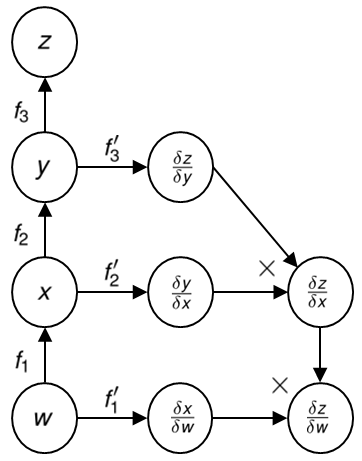
\includegraphics{figure/compgraph3}}% fit16:9 (was 0.25)
  \end{figure}
\end{frame}

\begin{frame} {Software for Deep Learning}
  \begin{wrapfigure}{R}{0.3\textwidth}
    \centering
      \scalebox{0.3}{
\includegraphics{figure/tflow.png}}
  \end{wrapfigure}
\textbf{Tensorflow}
\begin{itemize}
  \item Popular in the industry
  \item Developed by Google and \newline open source community
  \item Python, R, C++ and Javascript APIs
  \item Distributed training on GPUs and TPUs
  \item Tools for visualizing neural nets, running them efficiently on phones and embedded devices.
\end{itemize}

\begin{wrapfigure}{R}{0.3\textwidth}
  \centering
  \scalebox{0.3}{
\includegraphics{figure/keras.png}}
\end{wrapfigure}

\textbf{Keras}
  \begin{itemize}
    \item Intuitive, high-level \textbf{wrapper} on Tensorflow for rapid prototyping
    \item Python and (unofficial) R APIs
    
  \end{itemize}
\end{frame}

\begin{frame} {Software for Deep Learning}
  \begin{wrapfigure}{R}{0.3\textwidth}
    \centering
      \scalebox{0.3}{
\includegraphics{figure/pytorch.png}}
  \end{wrapfigure}

\textbf{Pytorch}
  \begin{itemize}
    \item Popular in academia
    \item Supported by Facebook
    \item Python and C++ APIs
    \item Distributed training on GPUs
  \end{itemize}

  \begin{wrapfigure}{R}{0.3\textwidth}
    \centering
      \scalebox{0.3}{
\includegraphics{figure/mxnet.png}}
  \end{wrapfigure}
  \vspace{3mm}
  \textbf{MXNet}
    \begin{itemize}
      \item Open-source deep learning framework written in C++ and cuda (used by Amazon for their Amazon Web Services) 
      \item Scalable, allowing fast model training
      \item Supports flexible model programming and multiple languages (C++, Python, Julia, Matlab, JavaScript, Go, \textbf{R}, Scala, Perl)
    \end{itemize}
\end{frame}


%%%%%%%%%%%%%%%%%%%%%%%%%%%%%%%%%%%%%%%%%%%%%%%%%%%%%%%%%%%%%%%%%%
\section{Hardware for Deep Learning: GPUs}
% Source: Stanford CS336 Spring 2025, lecture 5 (GPUs), slides 5-21, 45
% Text retypeset in the source's wording, figures cropped from the source PDF
%%%%%%%%%%%%%%%%%%%%%%%%%%%%%%%%%%%%%%%%%%%%%%%%%%%%%%%%%%%%%%%%%%

% CS336 lecture 5, slide 5
\begin{frame}{Setting the stage: compute leads to predictable perf}
\textbf{Often times, compute leads to predictable performance gains for language models}
\begin{center}
\includegraphics[page=5,trim=201 68 233 123,clip,width=\linewidth,height=108pt,keepaspectratio]{figure/cs336-l5.pdf}
\end{center}
\vspace{-0.6em}\par\hfill{\tiny Kaplan et al, Neural Scaling Laws}\par
Faster hardware, better utilization, improved parallelization alone can drive progress (for now..)
\end{frame}

% CS336 lecture 5, slide 6
\begin{frame}{How do we get compute scaling? Early on -- Dennard scaling}
\begin{center}
\includegraphics[page=6,trim=135 81 149 77,clip,width=\linewidth,height=128pt,keepaspectratio]{figure/cs336-l5.pdf}
\end{center}
But the traditional form of scaling (\emph{Dennard scaling}) from 1980-2000s has tapped out.\\
.. How do we feed LLMs' insatiable appetite for compute?
\end{frame}

% CS336 lecture 5, slide 7
\begin{frame}{Parallel scaling continues}
\begin{center}
\includegraphics[page=7,trim=144 95 149 75,clip,width=\linewidth,height=130pt,keepaspectratio]{figure/cs336-l5.pdf}
\end{center}
\vspace{-0.6em}\par\hfill{\tiny Bill Dally, HotChips keynote}\par
\begin{center}
Parallel scaling with GPUs has scaled $>$ 1000x in 10 years.\\
\emph{There is no LLM scaling without GPU scaling}
\end{center}
\end{frame}

% CS336 lecture 5, slide 8
\begin{frame}{How is a GPU different from a CPU?}
CPUs optimize for a few, fast threads while GPUs optimize for many many threads
\begin{columns}[T]
\begin{column}{0.55\textwidth}
\centering
\includegraphics[page=8,trim=37 103 312 114,clip,width=\linewidth]{figure/cs336-l5.pdf}\\[0.3em]
\small Many tiny compute units (ALUs).\\ Much less support for branching (control, cache)
\end{column}
\begin{column}{0.45\textwidth}
\centering
\vspace{1.6em}
\includegraphics[page=8,trim=420 140 30 184,clip,width=\linewidth]{figure/cs336-l5.pdf}\\[0.8em]
\small CPUs optimize for latency (each thread finishes quickly)\\
GPUs optimize for throughput (total processed data)
\end{column}
\end{columns}
\par\hfill{\tiny \url{https://developer.nvidia.com/blog/cuda-refresher-reviewing-the-origins-of-gpu-computing/}}\par
\end{frame}

% CS336 lecture 5, slide 9
\begin{frame}{Anatomy of a GPU (execution units)}
\begin{center}
\includegraphics[page=9,trim=82 88 92 70,clip,width=\linewidth,height=108pt,keepaspectratio]{figure/cs336-l5.pdf}
\end{center}
\begin{columns}[T]
\begin{column}{0.5\textwidth}
Each SM further contains many \textbf{SPs} (streaming processor) that can execute `threads' in parallel
\end{column}
\begin{column}{0.5\textwidth}
GPUs have \emph{many} \textbf{SM} (streaming multiprocessors) that independently execute `blocks' (jobs).
\end{column}
\end{columns}
\end{frame}

% CS336 lecture 5, slide 10
\begin{frame}{Anatomy of a GPU (memory)}
\textbf{The closer the memory to the SM, the faster it is} -- L1 and shared memory is \emph{inside} the SM. L2 cache is on die, and global memory are the memory chips next to the GPU
\begin{center}
\raisebox{-0.5\height}{\begin{tabular}{@{}c@{}}\includegraphics[page=10,trim=63 159 471 140,clip,width=78pt]{figure/cs336-l5.pdf}\\[2pt]\includegraphics[page=10,trim=63 44 471 255,clip,width=78pt]{figure/cs336-l5.pdf}\end{tabular}}\hspace{6pt}%
\raisebox{-0.5\height}{\includegraphics[page=10,trim=270 43 71 135,clip,width=160pt]{figure/cs336-l5.pdf}}
\end{center}
\small SRAM (shared/cache memory) is much more expensive (100x) but $\sim$ 8x faster than DRAM (Global memory)
\end{frame}

% CS336 lecture 5, slide 11
\begin{frame}{Execution model of a GPU}
\begin{center}
\includegraphics[page=11,trim=99 151 143 68,clip,width=\linewidth,height=95pt,keepaspectratio]{figure/cs336-l5.pdf}
\end{center}
There are 3 important players in the execution model
\begin{description}
\item[Threads:] Threads `do the work' in parallel -- all threads execute the same instructions but with different inputs (SIMT).
\item[Blocks:] Blocks are groups of threads. Each block runs on a SM w/ its own shared memory.
\item[Warp:] Threads always execute in a `warp' of 32 consecutively numbered threads each.
\end{description}
\end{frame}

% CS336 lecture 5, slide 12
\begin{frame}{Memory model of a GPU}
\begin{center}
\includegraphics[page=12,trim=142 108 152 80,clip,width=\linewidth,height=135pt,keepaspectratio]{figure/cs336-l5.pdf}
\end{center}
Each thread can access its own register, and shared memory within the block.\\
\textbf{Information that goes across blocks need to be read/written to global memory (slow)}
\end{frame}

% CS336 lecture 5, slide 13
\begin{frame}{Side thread -- What about TPUs?}
GPUs, TPUs, and many other accelerators are at a high level, similar
\begin{columns}[c]
\begin{column}{0.7\textwidth}
\centering
\includegraphics[page=13,trim=140 83 178 100,clip,width=\linewidth]{figure/cs336-l5.pdf}
\end{column}
\begin{column}{0.3\textwidth}
\small A GPU has more SMs\\
TPUs has fewer TCs\\
(but similar matmul perf)
\end{column}
\end{columns}
\small
\textbf{Core structure} -- lightweight control, fast (big) matmul unit, fast memory.\\
Differences -- how the accelerators are networked (in the parallelism lecture)\\
\hspace*{4.8em}-- no warps (just blocks -- tradeoffs in matmul vs non-matmul)
\end{frame}

% CS336 lecture 5, slide 14
\begin{frame}{Strengths of the GPU model}
\begin{itemize}
\item Easily scales up hard workloads (by adding more SMs)
\item Easy (?) to program due to the SIMT model
\end{itemize}
\begin{center}
\includegraphics[page=14,trim=204 151 242 151,clip,width=\linewidth,height=60pt,keepaspectratio]{figure/cs336-l5.pdf}
\end{center}
\begin{itemize}
\item Threads are `lightweight' and can be stopped and started
\end{itemize}
\begin{center}
\includegraphics[page=14,trim=170 13 186 283,clip,width=\linewidth,height=60pt,keepaspectratio]{figure/cs336-l5.pdf}
\end{center}
\end{frame}

% CS336 lecture 5, slide 15
\begin{frame}{GPUs as fast matrix multipliers}
\begin{center}
\includegraphics[page=15,trim=111 92 143 77,clip,width=\linewidth,height=150pt,keepaspectratio]{figure/cs336-l5.pdf}
\end{center}
Early days of NVIDIA GPUs -- programmable shaders. Researchers hacked this to do matmuls
\end{frame}

% CS336 lecture 5, slide 16
\begin{frame}{New matmul hardware means matmuls are fast and special}
\begin{center}
\includegraphics[page=16,trim=187 94 194 77,clip,width=\linewidth,height=130pt,keepaspectratio]{figure/cs336-l5.pdf}
\end{center}
Tensor cores (introduced in V, T series) are specialized matrix multiplication circuits.\\
\centerline{\textbf{Matmuls are $>$10x faster than other floating point ops!}}
\end{frame}

% CS336 lecture 5, slide 17
\begin{frame}{Compute scaling is faster than memory scaling}
\begin{center}
\includegraphics[page=17,trim=134 100 145 78,clip,width=\linewidth,height=132pt,keepaspectratio]{figure/cs336-l5.pdf}
\end{center}
\vspace{-0.6em}\par\hfill{\tiny \url{https://medium.com/riselab/ai-and-memory-wall-2cb4265cb0b8}}\par
FLOPs scale faster than memory -- it's hard to keep our compute units fed with data!
\end{frame}

% CS336 lecture 5, slide 18
\begin{frame}{Recap: GPUs -- what are they and how do they work}
\begin{columns}[c]
\begin{column}{0.58\textwidth}
\begin{itemize}
\item GPUs are massively parallel -- same instructions applied across many workers
\vspace{2.2em}
\item Compute (and esp matmuls) have scaled faster than memory
\vspace{2.2em}
\item We have to respect the memory hierarchy to make things go fast.
\end{itemize}
\end{column}
\begin{column}{0.42\textwidth}
\centering
\includegraphics[page=18,trim=475 245 77 72,clip,width=0.75\linewidth]{figure/cs336-l5.pdf}\\[3pt]
\includegraphics[page=18,trim=475 135 77 182,clip,width=0.75\linewidth]{figure/cs336-l5.pdf}\\[3pt]
\includegraphics[page=18,trim=478 19 72 288,clip,width=0.75\linewidth]{figure/cs336-l5.pdf}
\end{column}
\end{columns}
\end{frame}

% CS336 lecture 5, slide 19
\begin{frame}{Part 2: Making ML workloads fast on a GPU}
\begin{center}
\includegraphics[page=19,trim=150 79 198 79,clip,width=\linewidth,height=150pt,keepaspectratio]{figure/cs336-l5.pdf}
\end{center}
Performance on a GPU can be complex, even for something as simple as a square matmul
\end{frame}

% CS336 lecture 5, slide 20
\begin{frame}{What makes ML workloads fast?}
\textbf{The roofline model}
\begin{center}
\includegraphics[page=20,trim=176 73 176 109,clip,width=\linewidth,height=140pt,keepaspectratio]{figure/cs336-l5.pdf}
\end{center}
Key to this section: \textbf{how do we avoid being memory bound?}
\end{frame}

% CS336 lecture 5, slide 21
\begin{frame}{How do we make GPUs go fast?}
\begin{enumerate}
\item \textbf{Control divergence (not a memory bottleneck..)}
\item \textbf{Low precision computation}
\item \textbf{Operator fusion}
\item \textbf{Recomputation}
\item \textbf{Coalescing memory}
\item \textbf{Tiling}
\end{enumerate}
\end{frame}

% CS336 lecture 5, slide 45
\begin{frame}{Recap of part 2: making ML workloads go fast}
\begin{columns}[c]
\begin{column}{0.55\textwidth}
\begin{itemize}
\item Reduce memory accesses
\begin{itemize}\item Coalescing \item Fusion\end{itemize}
\item Move memory to shared memory
\begin{itemize}\item Tiling\end{itemize}
\item Trade memory for compute/accuracy
\begin{itemize}\item Quantization \item Recomputation\end{itemize}
\end{itemize}
\end{column}
\begin{column}{0.45\textwidth}
\centering
\includegraphics[page=45,trim=438 228 72 85,clip,width=0.8\linewidth]{figure/cs336-l5.pdf}\\[3pt]
\includegraphics[page=45,trim=440 129 72 184,clip,width=0.8\linewidth]{figure/cs336-l5.pdf}\\[3pt]
\includegraphics[page=45,trim=490 12 107 284,clip,width=0.45\linewidth]{figure/cs336-l5.pdf}
\end{column}
\end{columns}
\end{frame}

%%%%%%%%%%%%%%%%%%%%%%%%%%%%%%%%%%%%%%%%%%%%%%%%%%%%%%%%%%%%%%%%%%
\begin{frame}{License \& Attribution}
\footnotesize
\begin{itemize}
\item \textbf{Software for Deep Learning} is copied from \textbf{Introduction to Deep Learning (I2DL)}, SLDS, LMU Munich, chapter \emph{Hardware and Software} --- licensed \textbf{CC BY 4.0}: \url{https://creativecommons.org/licenses/by/4.0/}.
\item \textbf{Hardware for Deep Learning: GPUs} is adapted from \textbf{Stanford CS336 \emph{Language Modeling from Scratch}}, Spring 2025, Lecture 5 (\emph{GPUs}) by Tatsunori Hashimoto, \url{https://github.com/stanford-cs336/spring2025-lectures} --- \textbf{Copyright 2025 Stanford University}, licensed under the \textbf{MIT License} (full notice in \texttt{\_sources/}). One frame per selected source slide, in the source's order; text retypeset in the source's wording, figures cropped from the source PDF with the credits the source gives.
\item Selection and every edit: \texttt{order.txt}. \textbf{Original to this course:} the learning goals.
\end{itemize}
\end{frame}

\endlecture
\end{document}
